\section{Theory}
More detailed information on the theory of the experiment can be found in the 'Staatsexamen' by Martin Meyer.\cite{Anleitung}
\subsection{Born-Oppenheimer-Approximation}
For molecules with two atoms the time-independent Schrödinger equation gives the eigenfunctions and eigenvalues. For these two interacting particles equation \ref{eqHam} defines the Hamilton operator.
\begin{equation}
	H=-\frac{\hbar^2}{2m}\nabla+\frac{q_aq_b}{r}
	\label{eqHam}
\end{equation}
As a approximate solution for the time-independent Schrödinger
\begin{equation}
	\Psi=\Psi_E\cdot\Psi_N 
\end{equation}
can be used. $\Psi_E$ and $\Psi_N$ are solutions of the separated eq.\ref{eqHam1} and \ref{eqHam2}.  These describes the movement of the electrons and the movement of the core separately. 
\begin{equation}
	H_E\Psi_E=(T_E+V_{EE}+V_{EN})\Psi_E=E_E\Psi_E
	\label{eqHam1}
\end{equation}
\begin{equation}
H_N\Psi_N=(T_N+V_{NN}+V_{E})\Psi_N=E_N\Psi_N
\label{eqHam2}
\end{equation}
This so called Born-Oppenheimer-Approximation can be used since the electrons move much faster than the cores duo to their huge mass. That also means the electrons can adapt very fast to new distance between the cores and are almost not affected by the movement of the cores.
\subsection{Franck-Condon-Principle}
The Franck-Condon-Principle works on a similar assumption as the Born-Oppenheimer-Approximation. The idea is that an electronic transitions happen so fast, that they don't affect the slow moving cores, which results in the straight lines from one potential to the other one in figure \ref{figFranck}.
The principle describes the likelihood of these transition which depend on how much the ground and the exited potential overlay. The Franck-Condom-Factor \ref{eqFranck} gives this probability. 
\begin{equation}
	FC(v_i,v_k)=|\int \Psi_{\textbf{vib}}(v_i)\Psi_{\textbf{vib}}(v_k)dR|^2
	\label{eqFranck}
\end{equation}
Here $\Psi_{\textbf{vib}}$ is the vibration wave function and $v_i$ and $v_k$ are the vibration numbers for the exited and ground state.
\begin{figure}[ht]
	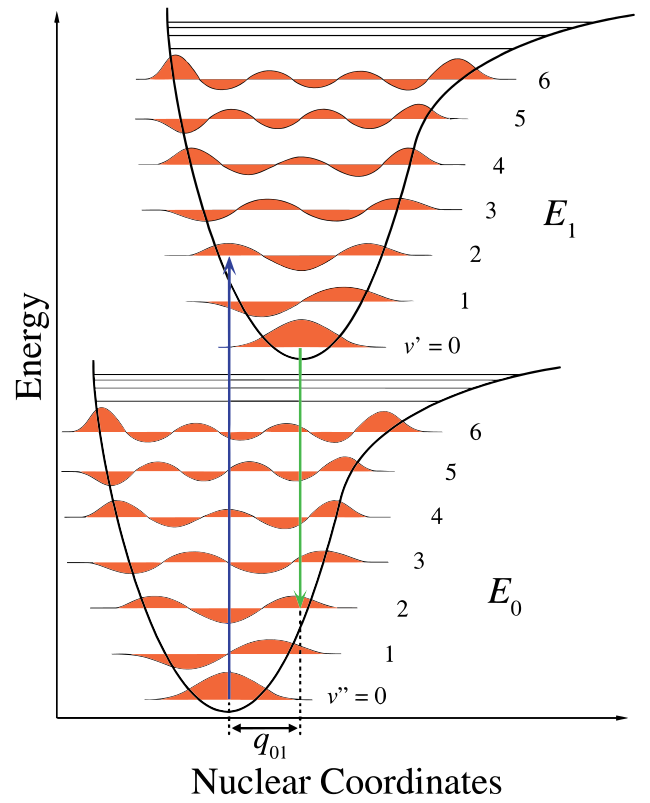
\includegraphics[scale=0.23]{Bild/FranckFaktor.png}
	\centering
	\caption[Franck-Condon-Principle]{\small Schematic representation of two atomic states with an example of two atomic molecules. The green and blue line represent the electronic transitions between these states, while the different vibration states $v'=v_i$ and $v''=v_k$ of the two states are in orange.\cite{Frank}}
	\label{figFranck}
\end{figure}
\FloatBarrier
\subsection{Morse Potential}
To describe an oscillation wave function without the rotation only the form of the potential energy is required. Often a harmonic potential is enough but especially for greater distances $R$ between the cores it shows huge differences to the real potential (see figure \ref{figPotential}). To describe the potential better for huge values of $R$ the Morse potential can be used. 
The Morse Potential is a anharmonic one and is defined by equation \ref{eqMorse}:
\begin{equation}
	E_{\textbf{Pot}}(R)=D_e\times[1-e^{-a(R-R_e)}]^2
	\label{eqMorse}
\end{equation}
Here $D_e$ is the potential depth or the dissociation energy, $a$ is a molecule constant, $R_e$ is the equilibrium bond distance and $R$ is the distance between the atoms.\par
The advantage of the Morse potential to a harmonic one is that it describes the real potential good for $R\Rightarrow \infty$ and for $R=R_e$. For $R\ll R_e$ the approximation is as good as a harmonic one. By using this equation to solve the Schrödinger equation, following 'eigenenergy' can be determined:
\begin{equation}
E_{\textbf{vib}}=\hbar \omega_e\left(v+\frac{1}{2}\right)-\hbar 	\omega_ex_e\left(v+\frac{1}{2}\right)^2 \qquad \text{with} \qquad \omega_ex=\frac{a^2\hbar}{4\pi c \mu} \qquad \qquad \omega_e=a\sqrt{\frac{\hbar D_e}{\pi c\mu}}
\end{equation}
With that the dissociation energy $D_e$ can be calculated using equation \ref{eqDis}:
\begin{equation}
	D_e=\frac{\omega_e^2}{4\omega_ex_e}
	\label{eqDis}
\end{equation}
With that the Morse potential gives the easiest extension of the harmonic oscillator by a term of the next higher order in the energy spectrum.
\begin{figure}[ht]
	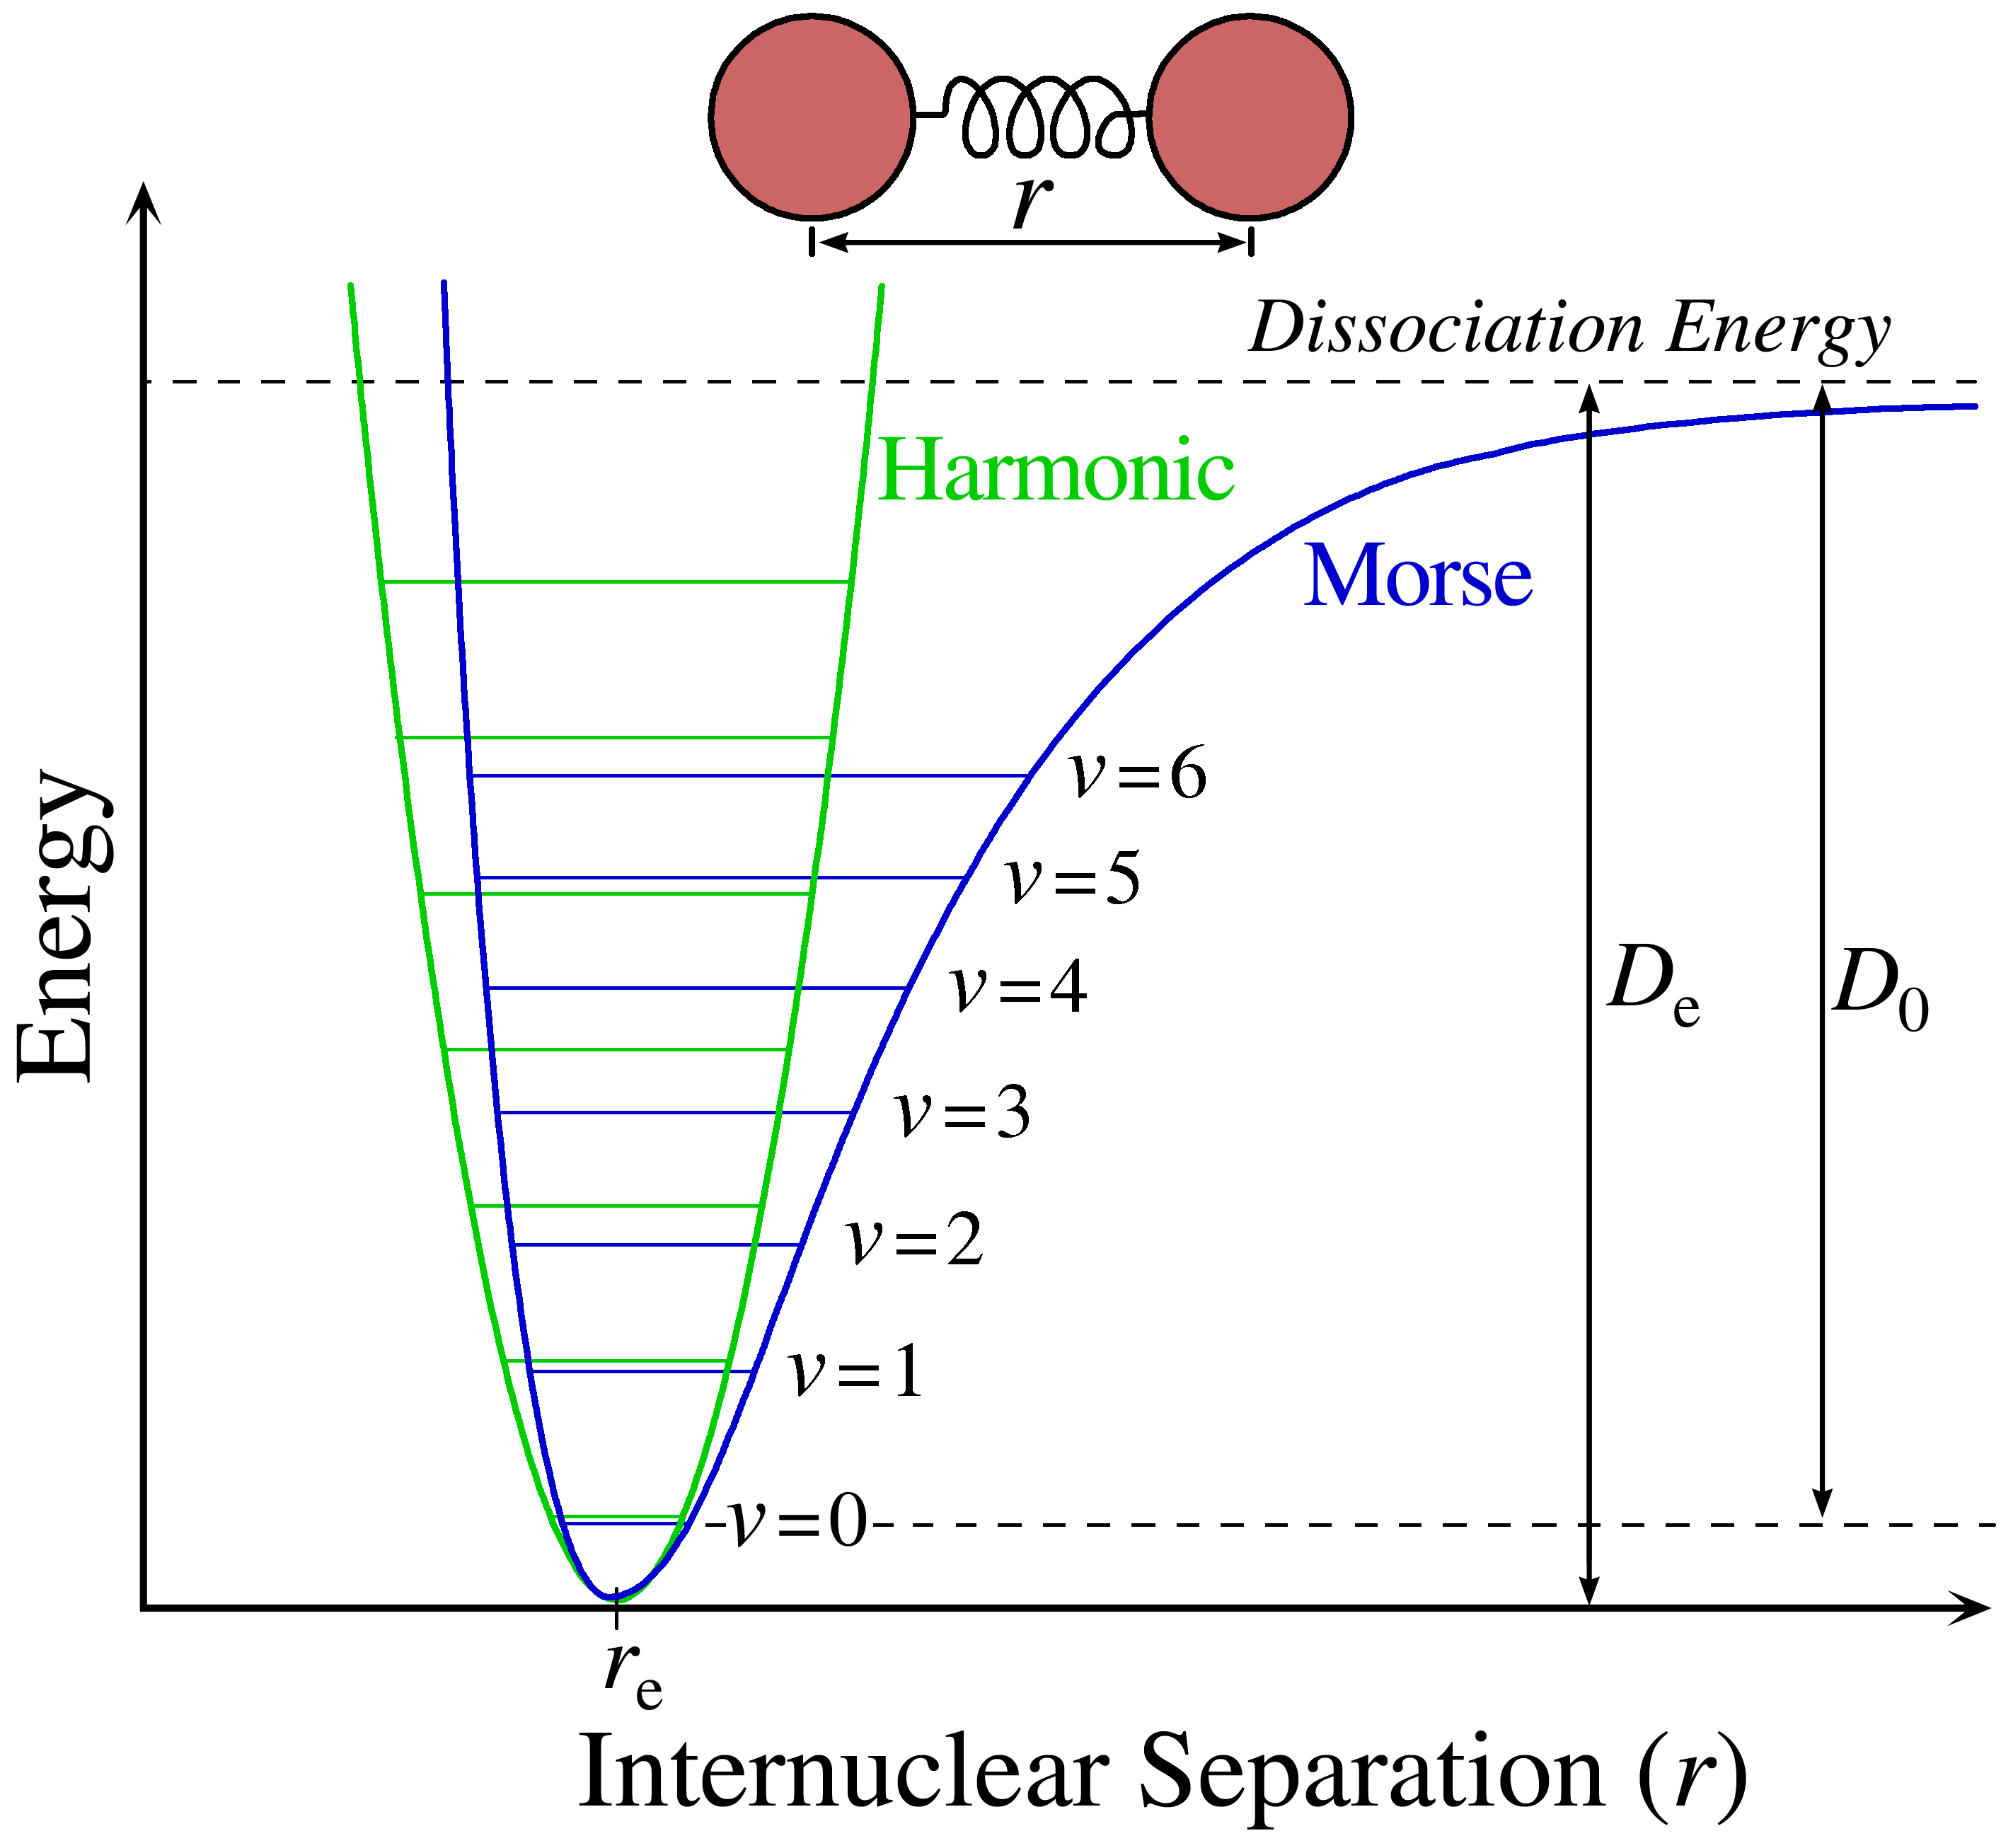
\includegraphics[scale=0.1]{Bild/Morse-potential.png}
	\centering
	\caption[Potential Forms]{\small Forms of the Morse in comparison to a Harmonic Potential. The dissociation or bonding energy $D_e$ which is higher than the energy $D_0$ which is needed to leave the potential.\cite{Morse}}
	\label{figPotential}
\end{figure}
\newpage
\subsection{Birge-Sponer-Plot}
The Birge-Sponer-Plot is a Method to calculate the dissociation energy $D_e$ as well as the values of $\omega_e$ and $x_e$.
Here we use the equation \ref{eqBSP} as equation of the different energy level by assuming an anharmonic oscillator. 
\begin{equation}
	G(v)=\frac{E_{\text{vib}}}{hc}=\omega_e(v+\frac{1}{2})-\omega_ex_e(v+\frac{1}{2})^2+\omega_ey_e(\frac{1}{2})^3+...
	\label{eqBSP}
\end{equation}
The differences between two adjusted energy levels is given by:
\begin{equation}
	\Delta G(v+\frac{1}{2})=G(v+1)-G(v)=\omega_e-\omega_ex_e(2v+2)+\omega_ey_e(3v^2+6v+\frac{13}{4})+...
	\label{DFaul}
\end{equation}
For an anharmonic potential the differences are getting smaller for higher $v$.
In the potential well the highest state at which the molecule dissociated is called $v_{dis}$. Above $G(v_{dis})$ is an energy continuum in which the molecule is dissociated (see fig.\ref{figCon}). Plotting $ G(v+\frac{1}{2})$ against $v+\frac{1}{2}$ is called the Birge-Sponer-Plot. With it and equation \ref{DFaul} the constants $\omega_e$ and $\omega_ex_e$ can be calculated. With them $D_e$ can be calculated using equation \ref{eqDis}.\par
Another way to get $D_e$ is to calculate the energy $D_0$ with the sum of the different energy distances $G(v+\frac{1}{2})$:\par
\begin{equation}
	D_0=\sum_{v=0}^{v_{dis}}\Delta G(v+\frac{1}{2})
	\label{D0}
\end{equation}
The dissociation energy $D_e$ is than:\par
\begin{equation}
	D_e=G(0)+D_0
	\label{De2}
\end{equation}
\begin{figure}[ht]
	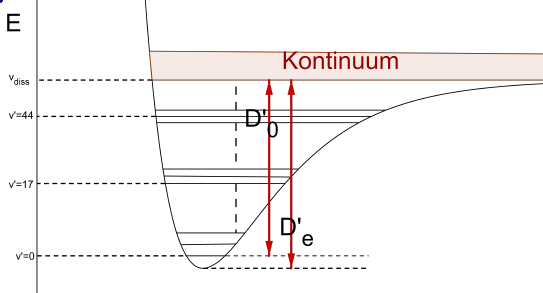
\includegraphics[scale=1.5]{Bild/PlotBirgeSponer.PNG}
	\centering
	\caption{Energy level with continuum and dissociation energy as well as $D_0$ that is smaller by $ G(0)$.\cite{Anleitung}}
	\label{figCon}
\end{figure}
\newpage
\subsection{Spectroscopic Notation and Transition Rules}
For the experiment the transition between the $I^2$ exited state and its ground state is used.
\begin{equation}
	X^1\Sigma^+_{0g}\leftrightarrow B^3\Pi^+_{0u}
\end{equation}
The notation of molecule states is normally in the form of:
\begin{equation}
	^{2S+1}\Lambda^{+/-}_{\Omega,u/g}
\end{equation}
\begin{enumerate}
	\item[-] $S$ being the quantum number of the total electron spin.
	\item[-] $\Omega$ is the projection of the total angular momentum $\vec{S}+\vec{L}$ on the molecular axis.
	\item[-] $+/-$ is the reflection symmetry along an arbitrary plane containing the internuclear axis.
	\item[-]$g/u$ is for  is the effect of the point group operation $\hat{i}$.
	\item[-]$\Lambda$ is the projection of the orbital angular momentum along the internuclear axis
\end{enumerate}
The letter $X$ stands for ground state and letters $(A,B,...)$ stands for exited states. For electronic dipole transitions there are the following rules:
\begin{enumerate}
	\item[-] $g\leftrightarrow u$, $g\nleftrightarrow g$, $g\nleftrightarrow g$
	\item[-] $\Delta \Omega=0,1,-1$
	\item[-] $\Delta \Lambda=0,1,-1$
	\item[-] $\Delta S=0$
\end{enumerate}
The reason why our transition doesn't contradicts these rules is the strong spin-orbit coupling. This acts as a perturbation that mixes states of different multiplicity.
\subsection{Iodine Tube}
The used iodine Tube is $50$\,cm long an has a radius of $2\,$cm and is filled with iodine. The Tube itself is inside a metal sheathing to eliminate stray light. At one side of the tube is a slit which can regulate the intensity of the light leaving the tube. For the experiment iodine is used since it has a broad absorption band system in the visible spectrum as well as the fact that there is only one stable iodine isotope.
\newpage
\subsection{CCD-Spectrometer}
A charged coupled device (CCD) is a device to that relies on the photo electric effect. It is made of a doped semiconductor. It saves the information of an incoming photons by create a electron, hole pair which can't drain off because of an applied voltage. By opening the potential well the saved electrons can be readout.\par
The CCD is only a part of the whole device which can be seen in figure \ref{figCCD}. It also has two mirrors to direct the incoming light and a lattice to create the spectrum. The CCD is only to read save the information which can be seen using the program \verb|SpectraSuit|. The used spectrometer has a slit width of $5\,\mu$m a wavelength range of $400-719\,$nm and a spectral resolution of $0.4\,$nm.
\begin{figure}[ht]
	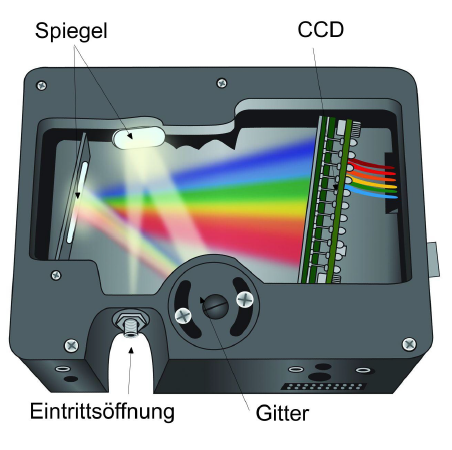
\includegraphics[scale=0.6]{Bild/CCD}
	\centering
	\caption[CCD-Spectrometer]{Structure of the CCD Spectrometer. The incoming light gets reflected on the lattice and from there to the CCD where the information is readout.\cite{Anleitung}}
	\label{figCCD}
\end{figure}
\FloatBarrier
\subsection{Monochromator}
The monochromator is used to get measure the spectrum of incoming light. The light gets reflected inside the device to a lattice which splits up the light into a spectrum. The light gets again reflected to the exited where a photometer is fixed. The lattice can be rotated with the help of the engine to pass through the spectrum. The Setup can be seen in figure \ref{figMono}.
In the input and exit of the monochromator are two slits to regulate the incoming and exiting light. It is important to note that the slit width should can be set betwenn $5\,\mu$m and $2000\,\mu$m, also the slit width can be set smaller this should never be done. To read the information the program \verb|JodAnalog| is used.
\begin{figure}[ht]
	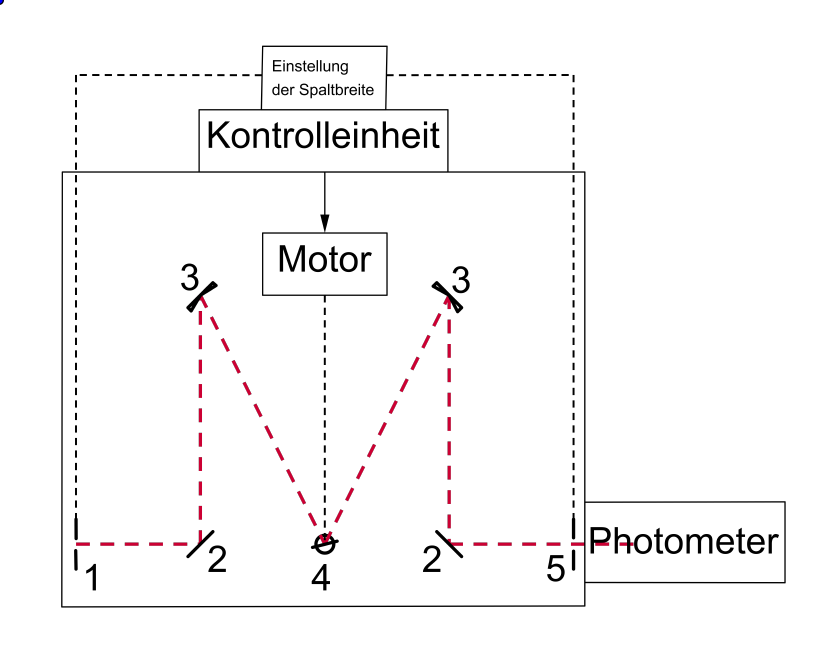
\includegraphics[scale=0.6]{Bild/Mono}
	\centering
	\caption[Monochromator]{Tis is a picture of the inside of the monochromator. $1$ and $5$ are the input and exit slits of the monochromator. With the help of the four mirrors $2$ and $3$ the light gets directed to exit and the lattice, which is at $4$.\cite{Anleitung}}
	\label{figMono}
\end{figure}